\documentclass{article}

\usepackage{iclr2025_conference}
\usepackage{times}
\usepackage{hyperref}
\usepackage{url}
\usepackage{booktabs}
\usepackage{amsfonts}
\usepackage{amsmath}
\usepackage{graphicx}
\usepackage{subcaption}
\usepackage{multirow}
\usepackage{xcolor}
\usepackage{float}
\iclrfinalcopy
\title{Detecting LLM-Generated Student Essays\\with Transformer Fine-Tuning and Cross-Domain Robustness Analysis}

\author{Joseph Souaiby - Huzaifah Wasim}

\begin{document}
\maketitle

\begin{abstract}
 In recent years, easy access to increasingly powerful large language models (LLMs) has made the reliable detection of AI-generated content in student writing critical for preserving academic integrity. In this project, we implement a transformer based detector and investigate its performance and generalization across dataset boundaries by performing cross-dataset evaluations. All models implemented, including the baselines, are trained on one corpus and tested out of distribution (OOD) on a second, statistically different dataset. We conduct full and Low-Rank Adaptation (LoRA) fine-tuning of RoBERTa with ranks 2,4, and 8 and benchmark them against TF-IDF and GLTR-style baselines on the "LLM Detect AI Generated Text" dataset from Kaggle and the RAID benchmark dataset. Each method achieves near perfect in domain accuracy (up to 99.95\%). However, Kaggle-trained models are observed to collapse to about 41\% accuracy in OOD evaluations on RAID, confirming that the models are memorizing dataset specific artifacts rather than learning patterns. In contrast, training on RAID substantially improves OOD accuracy when tested on the Kaggle dataset with LoRA rank 4 fine-tuning even outperforming full fine-tuning by 9.7\% achieving 59.9\% accuracy in OOD evaluations without meaningfully diminishing in-domain performance. Notably, this is achieved despite fine-tuning only about 0.12\% parameters compared to full fine-tuning. Our results confirm that a diverse training set and low-rank regularization are as at least as important as model capacity alone for robust AI-text detection.
\end{abstract}

\section{Introduction}
Large language models now produce fluent long-form writing that is increasingly difficult to distinguish from human-authored essays, which creates obvious risks for academic integrity. Numerous AI-text detectors have been proposed in recent years and benchmarks such as RAID \citep{dugan2024raid} are now being used to evaluate cross-domain performance. In this project, we study how training set compositions and parameter efficient fine tuning techniques such as LoRA affect OOD transfer. Specifically, we investigate whether LoRA's low rank constraints hinder or improve cross domain performance and robustness.

We formulate the task of AI detection as supervised binary classification. The input is just raw essay text and the target is a binary label. Formally, the labels are defined as $y \in \{0,1\}$. 0 and 1 signify human and AI written essays respectively. The models are trained by minimizing cross-entropy loss over the labels.

Our main model is a fine-tuned RoBERTa encoder with a linear classification layer. The model is trained and evaluated with RoBERTa fine tuned fully, with LoRA rank 2, rank 4, and rank 8. All the trained models are benchmarked against TF-IDF and GLTR encoding linear classifiers (SVM and Logistic Regression) using a cross dataset evaluation protocol using the Kaggle and RAID datasets. 

The question we specifically aim to answer is whether fine-tuned transformer based detectors generalize well on OOD samples across dataset boundaries and whether parameter efficient fine-tuning via LoRA diminishes or improves OOD robustness compared to full fine tuning? Our success criteria are: (1) achieving in-domain macro-F1 competitive with the best baseline trained on the same corpus, and (2) achieving higher OOD macro-F1 than any baseline or the fully fine-tuned model.

Reliable and effective cross-dataset detection matter now more than ever due to the ever increasing numbers of LLMs available. Our results show that even transformer based detection models collapse when subject to domain shift implying that multi-source training data, detector ensembles, or regularization strategies need to be employed by practitioners before deploying detectors in production. Fig \ref{fig:teaser} summarizes the full experimental pipeline and our code is publicly available at this \href{https://github.com/Joseph-Souaiby/DeepLearningProject.git}{link}.

\begin{figure}[H]
    \centering
    \includegraphics[width=0.5\linewidth]{figures/teaser_pipeline.pdf}
    \caption{TODO: Pipeline overview showing cross-dataset evaluation protocol and the
    LoRA rank--robustness finding.}
    \label{fig:teaser}
\end{figure}

% ===========================================================================
% 2  PROBLEM FORMULATION + RELATED WORK  (12 pts)
%   - Coverage of 3+ closely related lines of work: 4 pts
%   - Positioning (comparison table/paragraph clarifying contributions): 4 pts
%   - Description of problem with inputs/outputs and formulation: 4 pts
% ===========================================================================
\section{Problem Formulation and Related Work}

% --- Problem formulation (4 pts) ---
\subsection{Problem Formulation}
Our main task is training a detector $f_\theta(x) \rightarrow [0,1]$ that maps a raw essay $x$ to the probability that it is AI-generated. Our model receives tokenized text truncated to 512 tokens as input using which it outputs a two class logit vector $z$. This is then piped to a softmax layer to calculate the predicted probability $\hat{y} = \mathrm{softmax}(z)$. The target variable is a binary label $y \in \{0,1\}$ where $0=human$ and $1=AI$. The training minimizes the cross entropy loss:
\begin{equation}
\mathcal{L}_{\text{CE}} = -\frac{1}{N}\sum_{i=1}^{N}\left[y_i \log \hat{y}_i
+ (1 - y_i)\log(1 - \hat{y}_i)\right]
\label{eq:ce}
\end{equation}
where $\hat{y}_i$ is the predicted probability that essay $i$ is
AI-generated.

The model is then evaluated in-domain and OOD using metrics of accuracy, macro-F1, class-wise precision and recall, and AUROC. Macro-F1 is the main metric as it is invariant to class imbalances

\subsection{Related Work}
Both likelihood-based
heuristics and supervised representation learning have been used to help detect AI generated content. GLTR \citep{gehrmann2019gltr} shows that token-rank statisticscan help expose generation based artifacts. DetectGPT
\citep{mitchell2023detectgpt} proposes a training-free signal based on observing the
curvature of log-likelihood while perturbing. GLTR's ability to capture generation artifacts without relying on sparse word overlap is what motivated us to use it as a baseline. Our baseline builds on
this by aggregating 16 essay-level likelihood statistics from
DistilGPT-2 and feeding them into an SVM and logictic regression linear classifier.

For supervised detection, transformer encoders such as BERT
\citep{devlin2019bert} and RoBERTa \citep{liu2019roberta} provide
strong representations for document classification, with RoBERTa being
the natural choice for our main model. This
however, does not automatically imply robustness to generator or
domain shift. Benchmark papers such as TURINGBENCH \citep{uchendu2021turingbench} and HC3 \citep{guo2023close} show that
detectors' performance transfer across domains and on different generators remains difficult. We chose RAID \citep{dugan2024raid} because it addresses this by providing a multi-generator, multi-domain benchmark for cross-domain evaluation. We use RoBERTa-base as our primary encoder and leverage both Kaggle and RAID corpora in a symmetric cross-dataset protocol to
directly test OOD transfer.

Low Rank Adaptation (LoRA) uses trainable low-rank decomposition matrices into the frozen transformer layers \citep{hu2022lora}. This helps reduce the number of trainable parameters while preserving competitive task performance. LoRA has not been systematically studied as a regularization technique for generalized cross-domain AI-text detection. We investigate whether low-rank constraints resolve RoBERTa's tendency to memorize dataset/text specific lexical artifacts rather than learning generator distributions. This would potentially improve OOD robustness without meaningful in-domain reduction in performance.

Table \ref{tab:positioning} summarizes our work's relation to prior approaches. We found that no existing study combines transformer fine tuning, OOD evaluation, LoRA, and AI detection. 
\begin{table}[H]
\centering
\caption{Positioning relative to prior work.}
\label{tab:positioning}
\small
\begin{tabular}{@{}lccc@{}}
\toprule
Work & OOD Eval & LoRA Ablation & Cross-Dataset \\
\midrule
GLTR & \texttimes & \texttimes & \texttimes \\
DetectGPT & \texttimes & \texttimes & \texttimes \\
TURINGBENCH & \checkmark & \texttimes & \texttimes \\
HC3 & Partial & \texttimes & \texttimes \\
\textbf{Ours} & \checkmark & \checkmark & \checkmark \\
\bottomrule
\end{tabular}
\end{table}

\section{Method and Approach}

\subsection{Research Hypotheses}

We have structured our experiments to test 3 main hypothesis:

\textbf{H1:} Fine-tuned RoBERTa encoder will outperform TF-IDF and GLTR based classifier baselines in-domain on the Kaggle dataset, measured by macro-F1 and AUROC using the same train/validation/test split. We compare full fine-tuned RoBERTa against all baselines. We expect full fine-tuned RoBERTa to outperform all four baselines. This is because transformers have the ability to capture writing patterns and relations in text that aggregate likelihood based (GLTR) or bag-of-words (TF-IDF) mehods cannot capture.

\textbf{H2:} Training RoBERTa on the multi-generator RAID dataset will achieve better OOD transfer (higher macro-F1) when tested on the Kaggle dataset compared to training on the Kaggle dataset and testing OOD performance on RAID. We predict this because RAID is much more diverse and will encourage the model to learn generator-invariant features rather than memorizing source specific lexical artifacts that can not be relied upon across dataset boundaries.

\textbf{H3:} We predict that parameter efficient fine tuning (LoRA) will match full fine-tuning wihin 2 macro-F1 points in in-domain testing and achieve a higher OOD macro-F1 than full tine-tuning. This is because the low-rank constraint helps prevent the model from memorizing domain specific patterns. Furthermore, we hypothesize that there is a rank of LoRA below full fine-tuning that will maximize OOD macro-F1. Ranks that are too low will underfit. We test this by conducting a rank sweep over $r\in \{2.4.8\}$ plus a frozen version of RoBERTa and full fine tuned version as boundary conditions. All will be trained on RAID and OOD evaluations will be conducted on the Kaggle dataset
\subsection{Model Architecture}

We use RoBERTa-base encoder \citep{liu2019roberta} (124M parameters) paired with a classification head consisting of a dropout layer ($p=0.1$) followed by a linear layer with a 768 dimension input, outputting 2 logits. We use both the logits and embeddings returned by the model for our analysis.

We use the HuggingFace PEFT library to apply LoRA \citep{hu2022lora} for parameter efficient fine tuning, inserting low rank decomposition matrices across all 12 transformer layers. We then train different models while sweeping over ranks $r \in \{2, 4, 8\}$ with $\alpha = 2r$ and LoRA dropout of 0.1.

We included full parameter fine tuning and the frozen RoBERTa with only the classification head trained as boundary conditions. The parameter counts can be seen in Table 2 below:

\begin{table}[H]
\centering
\caption{Training configurations.}
\label{tab:params}
\small
\begin{tabular}{@{}lrr@{}}
\toprule
Configuration & Trainable Params & \% of Total \\
\midrule
Full fine-tuning & 124,645,632 & 100\% \\
LoRA $r=8$ & 294,912 & 0.236\% \\
LoRA $r=4$ & 147,456 & 0.118\% \\
LoRA $r=2$ & 73,728 & 0.059\% \\
Frozen backbone & $\sim$1,538 & $\sim$0.001\% \\
\bottomrule
\end{tabular}
\end{table}
\subsection{Training Details}
All the RoBERTa configurations were trained using the AdamW optimizer with a weight decay of $0.01$ and gradient clipping at max norm $1.0$. For full fine tuning and frozeen RoBERTa we used a differential learning rate of $2 \times 10^{-5}$ for the encoder and $1 \times 10^{-3}$ for
the classification head. For all LoRA configurations we used a constant learning rate of $2 \times 10^{-4}$. We used a batch size of 32. The input text is cleaned and tokenized using  HuggingFace \texttt{AutoTokenizer} and truncated to 512 toens. We then use \texttt{DataCollatorWithPadding} to handle padding in each batch. Cross entropy is used as the minimization objective for all configurations.

\subsection{Design Justification}
Our decision to choose RoBERTa over Vanilla BERT (V-BERT) was motivated by three main advantages of RoBERTa over V-BERT: its improved pretraining with dynamic masking, no next sentence prediction objective, and a larger training dataset which all lead to better performance on text classification tasks. The decision to apply LoRA to the attention and query modules stemmed from \citet{hu2022lora} identifying those modules as the most parameter efficient subset. The encoder learning rate is chosen to be small to prevent to much parameter deviation from pretrained weights. The rank sweep $r \in \{2, 4, 8\}$ is designed to test the models in light of H3. The frozen version of RoBERTa serves as a lower bound answering the question that if pretrained representations alone are enough for detection then fine tuning is unnecessary.
\subsection{Evaluation Strategy}
All models are tested using the cross-dataset OOD method. Models trained on the Kaggle dataset are tested in-domain on a test split and on a balanced 10,000 sample RAID dataset. Models trained on RAID are tested in domain on a RAID test set and OOD evaluations are conducted on the Kaggle dataset. We measure and report accuracy, macro-F1, class-wise precision and recall, AUROC, confusion matrices, and ROC curves. All baselines are evaluated using the same exact protocol to ensure a fair comparison. 
\subsection{Reproducibility}
We performed all the experiments on Google Colab with a single NVIDIA A100 GPU. We used PyTorch 2 with HuggingFace for tokenizing, padding, LoRA, and data loading. All hyperparameters are reported in previous sections. All code is publicly available on GitHub: \url{https://github.com/Joseph-Souaiby/DeepLearningProject.git}

\section{Data}

% --- Dataset description (4 pts) ---
\subsection{Dataset Description}
We used two different datasets for this project: \href{https://www.kaggle.com/datasets/sunilthite/llm-detect-ai-generated-text-dataset}{The Kaggle Dataset "LLM Detect AI Generated Text"} and the \href{https://huggingface.co/datasets/liamdugan/raid}{RAID Benchmark Dataset}

The Kaggle dataset contains student and AI-generated essays on fixed prompts. After cleaning the dataset contained 27,278 essays with a class distribution of 59\% human and 42\% AI generated essays. The dataset has binary labels with 0 representing human and 1 representing AI. This dataset uses a single generator to generate the essays.

Unlike the Kaggle dataset, RAID \citep{dugan2024raid} is a multi-generator, multi-domain dataset which we sourced from HuggingFace. The target labels in RAID are generator names or "human". We relabeled the dataset with a binary scheme exactly the same as the Kaggle dataset. After binarizing the labels, we noticed a major class imbalance in the dataset. It had 96\% AI generated texts and only 4\% human generated texts. We mitigated this by resampling 100,000 samples from the dataset leading to a 29\% and 71\% class distribution for human and AI labels respectively. For OOD evaluations we constructed a separate unsplit 10,000 sample subset of RAID. Table \ref{tab:data} summarizes the statistics.


\subsection{Preprocessing and Splits}
Both datasets were preprocessed and split using the exact same pipeline which consisted of whitespace normalization, de-duplication, and a 50-char minimum length filter. All these steps were applied before splitting. 

Both datasets are split in ratios of 0.7/0.1/0.2 using stratified sampling. Kaggle had a train/val/test split of 19,094/2,728/5,456 and RAID yields 69,999/10,000/20,000. For RoBERTa models we tokenized the essays using \texttt{AutoTokenizer}, truncated to 512 tokens, and dynamically padded via \texttt{DataCollatorWithPadding}.
\begin{table}[H]
\centering
\caption{Dataset statistics after cleaning and splitting.}
\label{tab:data}
\small
\begin{tabular}{@{}lrrrrrr@{}}
\toprule
Dataset & Total & Human & AI & Train & Val & Test \\
\midrule
Kaggle & 27,278 & 16,098 & 11,180 & 19,094 & 2,728 & 5,456 \\
RAID (train) & 100,000 & $\sim$14k & $\sim$86k & 69,999 & 10,000 & 20,000 \\
RAID (OOD eval) & 10,000 & 5,900 & 4,100 & \multicolumn{3}{c}{--- eval only ---} \\
\bottomrule
\end{tabular}
\end{table}


\section{Experiments and Results}

% --- Baselines (6 pts) ---
\subsection{Baselines}
For our baselines, we observed that TF-IDF has almost perfect in-domain performance on the Kaggle test set and it achieves 99.74\% accuracy with SVM. However, it collapses horribly on RAID OOD with only 41\% accuracy, macro-F1 of just 0.29, human recall of 0 meaning that TF-IDF generates false positives for all human essays as being AI generated. While GLTR is weaker than TF-IDF in-domain with 95.64\% accuracy, it has much better OOD performance on RAID reaching 57.78\% accuracy and 0.56 macro-F1 with a logistic regression classifier. This makes it clear that GLTR is able to learn features in generated text that generalize better than TF-IDF's bag-of-words approach. A summary of baseline results can be seen in Table \ref{tab:baselines} below
\begin{table}[H]
\centering
\caption{Baseline results on Kaggle (in-domain) and RAID (OOD).}
\label{tab:baselines}
\small
\begin{tabular}{@{}llcccc@{}}
\toprule
Eval Set & Method & Acc.\,(\%) & Macro-F1 & Human Rec. & AI Rec. \\
\midrule
Kaggle & TF-IDF + LogReg & 99.12 & 0.99 & 1.00 & 0.98 \\
Kaggle & TF-IDF + SVM & 99.74 & 1.00 & 1.00 & 0.99 \\
Kaggle & GLTR + LogReg & 95.42 & 0.95 & 0.95 & 0.96 \\
Kaggle & GLTR + SVM & 95.64 & 0.96 & 0.96 & 0.96 \\
\midrule
RAID & TF-IDF + LogReg & 40.86 & 0.29 & 0.00 & 1.00 \\
RAID & TF-IDF + SVM & 40.90 & 0.29 & 0.00 & 0.99 \\
RAID & GLTR + LogReg & 57.78 & 0.56 & 0.30 & 0.97 \\
RAID & GLTR + SVM & 55.20 & 0.52 & 0.26 & 0.97 \\
\bottomrule
\end{tabular}
\end{table}

% --- RoBERTa + LoRA results and ablations (6 pts) ---
\subsection{Transformer Results and Ablations}
Full fine tuned RoBERTa encoder plus linear classifier achieves even better in-domain performance than TF-IDF+SVM with 99.95\% accuracy on the Kaggle dataset. However, just like TF-IDF it collapses to 42.79\% accuracy on RAID OOD evaluation. LoRA with $r{=}8, \alpha{=}16$ shows the same high in-domain and OOD collapse pattern  with 99.16\% and 40.97\% accuracy respectively. This confirms that when training data lacks diversity, throwing more power at the problem will not help generalization.

Training RoBERTa on RAID substantially improves performance. Full fine tuned RoBERTa achieves 94.06\% in domain accuracy while still collapsing on Kaggle OOD evaluation to a 7.4pp higher  50.22\% compared to kaggle-trained full fine tuned RoBERTa. 

The most interesting results arise from LoRA rank sweep training on RAID and OOD evaluation on Kaggle. We see a non-monotonic pattern emerge starting from frozen RoBERTa which achieves only 41.29\% OOD accuracy, LoRA ($r{=}2,\alpha{=}4$) rises to 51.98\% accuracy, LoRA ($r{=}4, \alpha{=}8$) peaks at
59.90\%, LoRA ($r{=}8, \alpha{=}16$) drops back to 56.89\%, and full fine tuned RoBERTa drops further to 50.22\%. In contrast, and predictably, in-domain accuracy rises almost monotonically with number of  training parameters. Starting with frozen RoBERTa achieving 81.47\%, LoRA-2 achieving 89.81\%, LoRA-4 reaching 93.94\%, LoRA-8 achieving 93.62\% and full fine tuned RoBERTa reaching 94.06\% accuracy. This confirms that the fact that OOD peaks at LoRA ($r=4$) is not due to better in-domain learning. Figure \ref{fig:rank_sweep} shows the concave accuracy curve of OOD evaluations on Kaggle against trainable parameters. Table \ref{tab:summary} presents the metrics for all 11 models trained and tested in this project

Figure \ref{fig:ood_cm} shows our failure modes. Specifically, all kaggle trained models fail by defaulting to predicting AI on OOD data, generating false positives and reducing human recall to almost zero. This indicates that models are unable to learn patterns in human writing, rather they are memorizing what Kaggle AI essays look like. Figure \ref{fig:best_model} shows that even the best model drops human recall from 0.83 in-domain
to 0.32 OOD.
\begin{table}[H]
\centering
\caption{Cross-dataset results. All models evaluated both in-domain
and OOD}
\label{tab:summary}
\small
\begin{tabular}{@{}llccccc@{}}
\toprule
Model & Train & Train.\,\% & ID Acc & ID F1 & OOD Acc & OOD F1 \\
\midrule
TF-IDF + LogReg & Kaggle & --- & 99.12 & 0.99 & 40.86 & 0.29 \\
TF-IDF + SVM & Kaggle & --- & 99.74 & 1.00 & 40.90 & 0.29 \\
GLTR + LogReg & Kaggle & --- & 95.42 & 0.95 & 57.78 & 0.56 \\
GLTR + SVM & Kaggle & --- & 95.64 & 0.96 & 55.20 & 0.52 \\
\midrule
RoBERTa Full FT & Kaggle & 100 & 99.95 & 1.00 & 42.79 & 0.37 \\
LoRA $r{=}8$ & Kaggle & 0.24 & 99.16 & 0.99 & 40.97 & 0.32 \\
\midrule
RoBERTa Full FT & RAID & 100 & 94.06 & 0.93 & 50.22 & 0.45 \\
LoRA $r{=}8$ & RAID & 0.24 & 93.62 & 0.92 & 56.89 & 0.54 \\
\textbf{LoRA $r{=}4$} & \textbf{RAID} & \textbf{0.12} & \textbf{93.94} & \textbf{0.92} & \textbf{59.90} & \textbf{0.58} \\
LoRA $r{=}2$ & RAID & 0.06 & 89.81 & 0.86 & 51.98 & 0.47 \\
Frozen & RAID & $<$0.01 & 81.47 & 0.72 & 41.29 & 0.30 \\
\bottomrule
\end{tabular}
\end{table}

% ----- FIGURE 2: OOD CONFUSION MATRICES (6 pts: failure modes) -----
% PURPOSE: Directly earns "failure modes" component of the 6-pt visualization criterion.
%          Shows the class-asymmetric collapse pattern: all Kaggle-trained models default to
%          predicting AI on OOD data, collapsing human recall to ~0.
% WHY THESE 3: TF-IDF shows the worst collapse (0.00 human recall), GLTR shows partial
%          recovery (0.30 human recall), and RoBERTa shows that a more powerful model does NOT
%          fix the problem (0.10 human recall). This trio tells the story that architecture
%          alone cannot overcome training-distribution bias.
% SOURCE: Google Drive folders — download confusion_matrix.png from each
\begin{figure}
    \centering
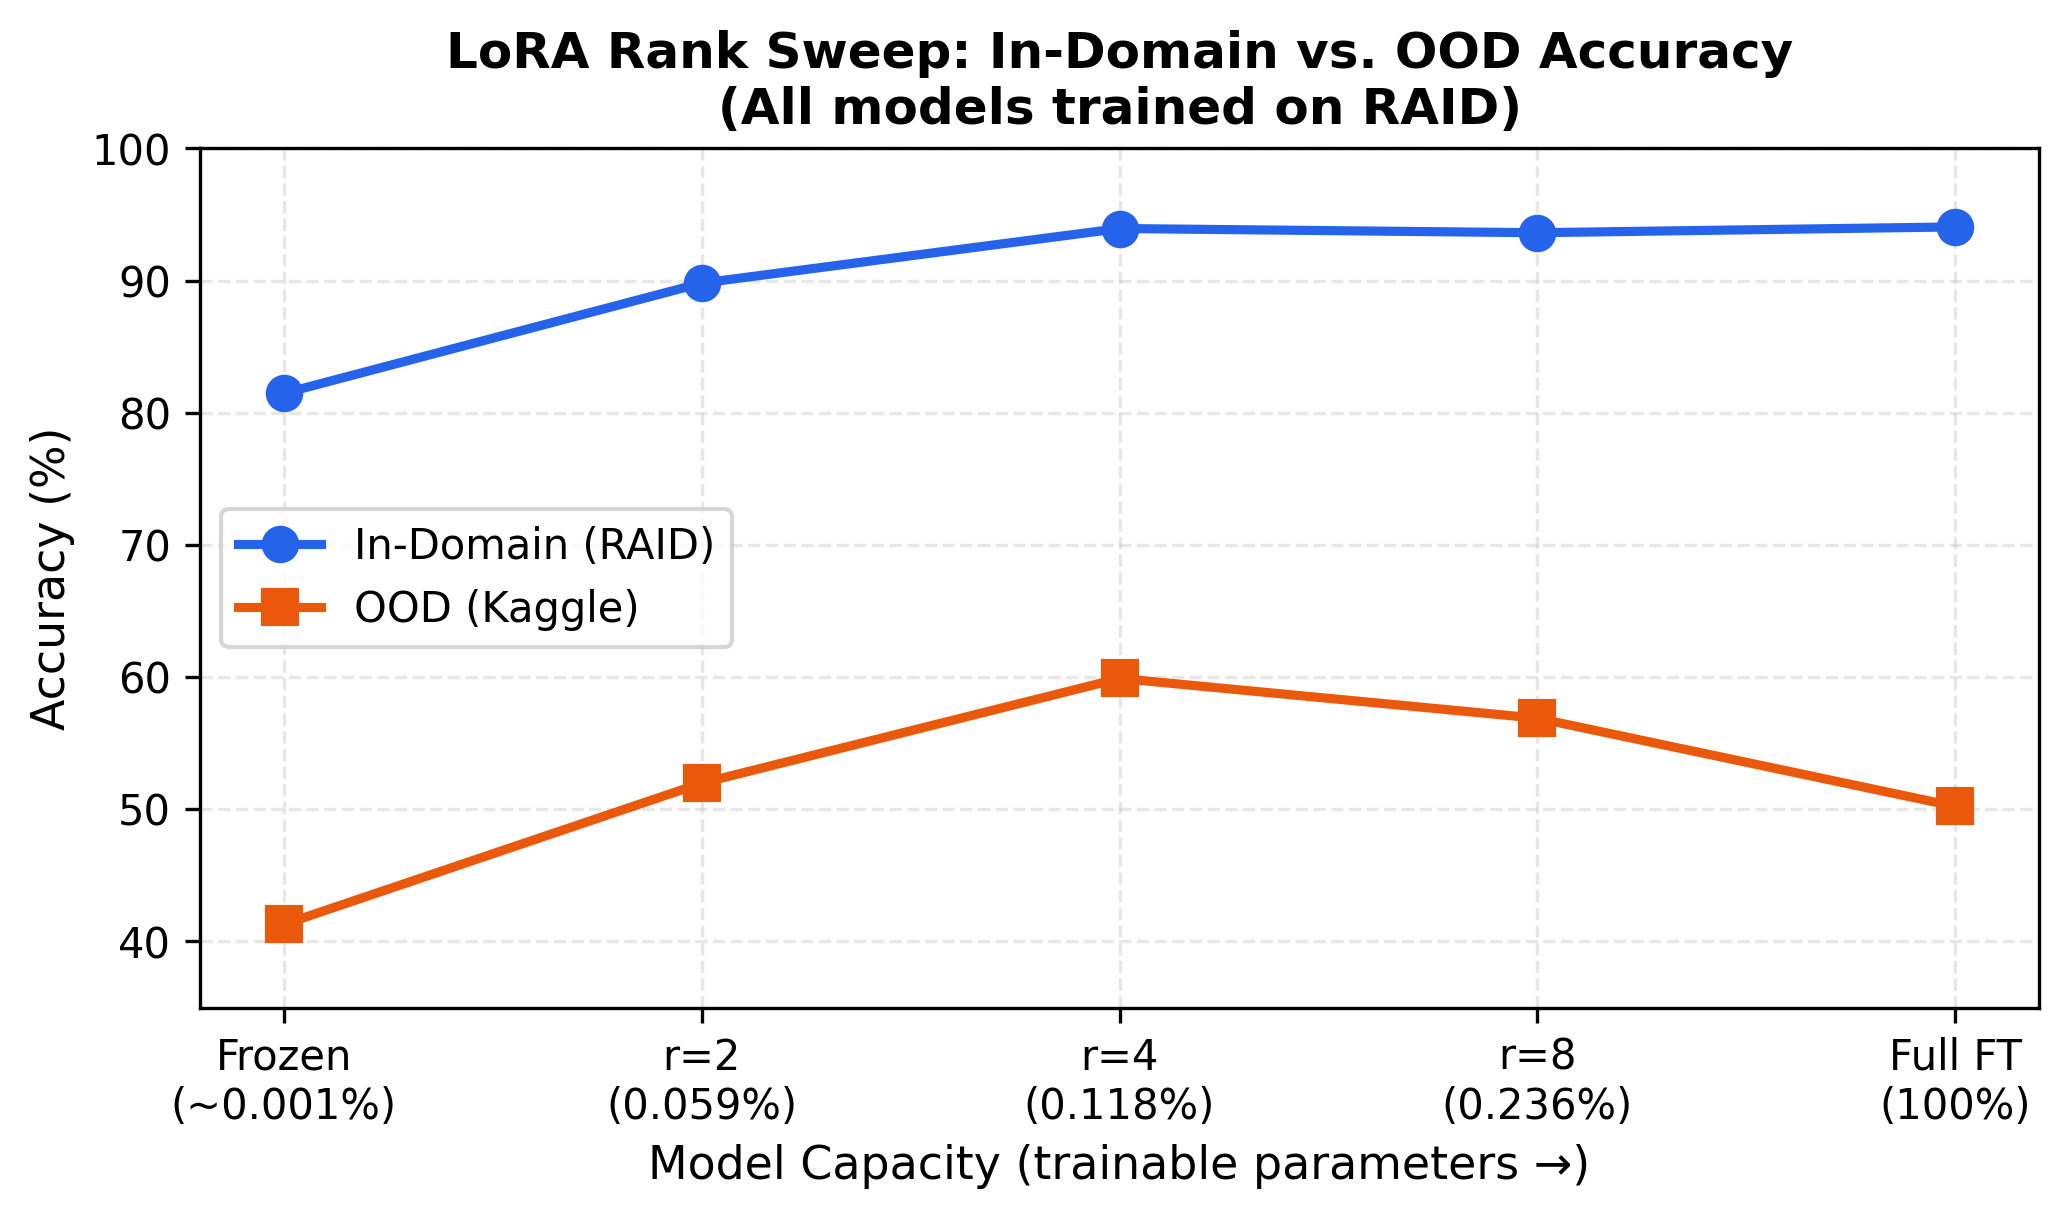
\includegraphics[width=0.7\linewidth]{results/lora_rank_sweep.png}
    \caption{LoRA rank sweep for RAID-trained models.}
    \label{fig:rank_sweep}
\end{figure}

\begin{figure}[H]
    \centering
    \begin{subfigure}[b]{0.3\linewidth}
        
\includegraphics[width=\linewidth]{results/raid_log_reg/confusion_matrix.png}
        \caption{TF-IDF LogReg on RAID}
    \end{subfigure}
    \hfill
    \begin{subfigure}[b]{0.3\linewidth}
        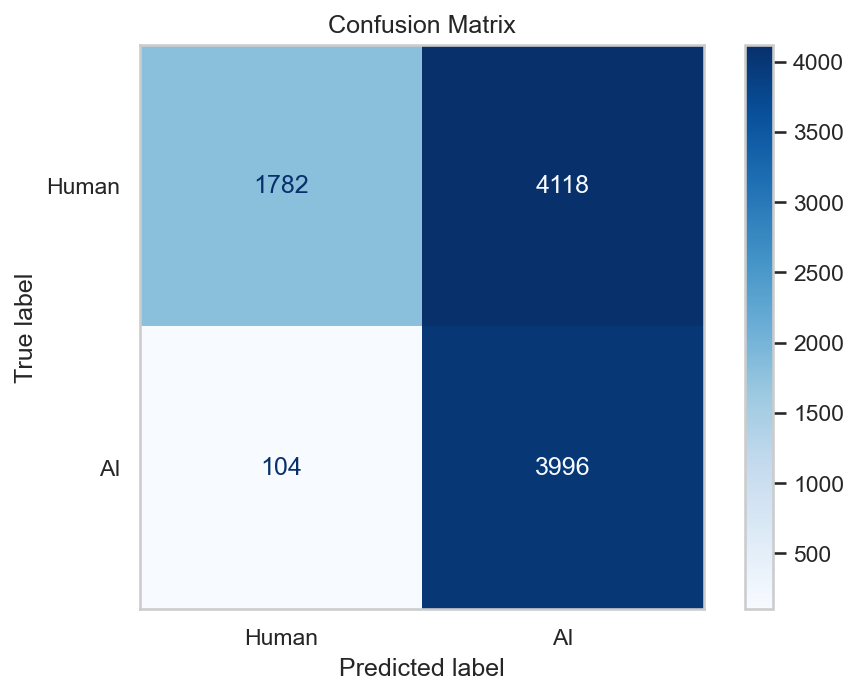
\includegraphics[width=\linewidth]{results/raid_gltr_log_reg/confusion_matrix.png}
        \caption{GLTR LogReg on RAID}
    \end{subfigure}
    \hfill
    \begin{subfigure}[b]{0.3\linewidth}
        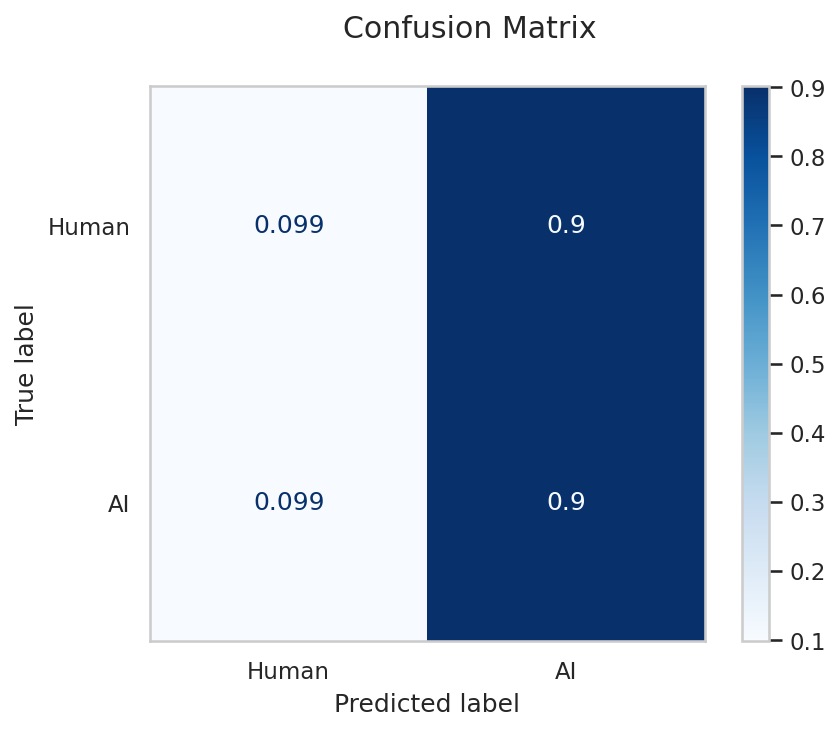
\includegraphics[width=\linewidth]{results/roberta_kaggle_raid/confusion_matrix.png}
        \caption{RoBERTa Full FT on RAID}
    \end{subfigure}
    \caption{OOD confusion matrices for Kaggle-trained models evaluated on RAID}
    \label{fig:ood_cm}
\end{figure}

% ----- FIGURE 3: LoRA RANK SWEEP (6 pts: ablations) -----
% PURPOSE: Earns "ablations" points and provides the key visual evidence for H3.
%          A line plot with LoRA rank on x-axis and two lines (in-domain RAID accuracy
%          and OOD Kaggle accuracy). Shows the non-monotonic OOD curve peaking at r=4.
% WHY NOT A TABLE: The non-monotonic shape is the insight — a line plot reveals
%          the curve shape immediately, while a table hides it.
% SOURCE: You generate this from the results data. X-axis: Frozen, r=2, r=4, r=8, Full FT.
%         Y-axis: accuracy. Two lines: RAID in-domain, Kaggle OOD.


% ----- FIGURE 4: BEST MODEL IN-DOMAIN vs OOD (6 pts: analysis) -----
% PURPOSE: Earns the "analysis" component of the visualization criterion.
%          Shows that even the BEST model (LoRA r=4) still has a 34 pp OOD gap.
%          The side-by-side comparison of the same model on two datasets directly
%          visualizes the transfer problem and motivates future work.
% WHY NOT ROC CURVES: ROC curves all show AUC ~0.99 in-domain, which is redundant with
%          the tables. These paired CMs are more informative — they show WHERE
%          the model fails (human recall drop) rather than just aggregate discrimination.
% SOURCE: Google Drive — download confusion_matrix.png from each folder
\begin{figure}[H]
    \centering
    \begin{subfigure}[b]{0.4\linewidth}
        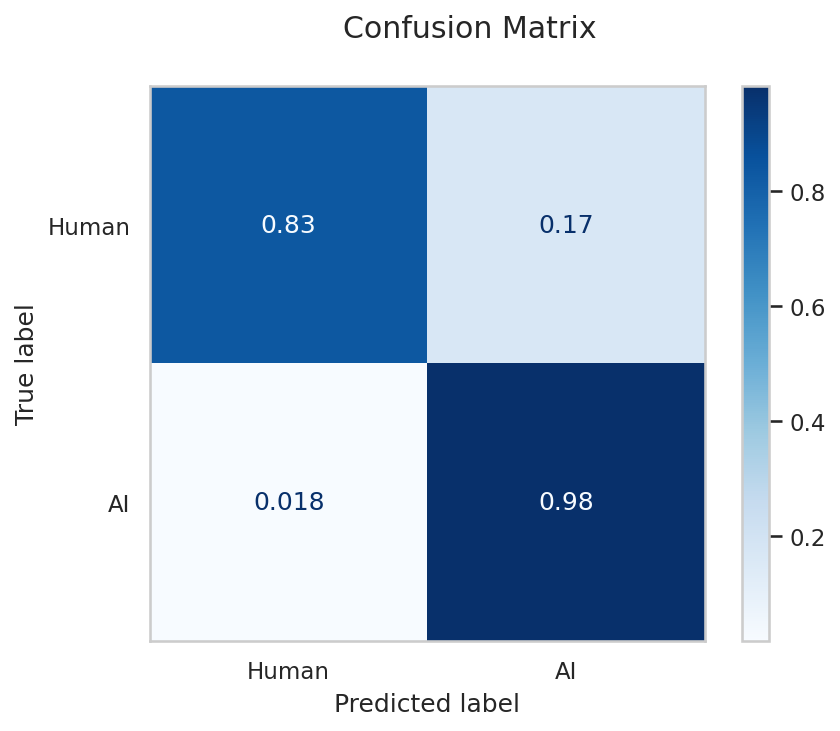
\includegraphics[width=\linewidth]{results/lora_raid_raid_4/confusion_matrix.png}
        \caption{In-domain (RAID test set)}
    \end{subfigure}
    \hfill
    \begin{subfigure}[b]{0.4\linewidth}
        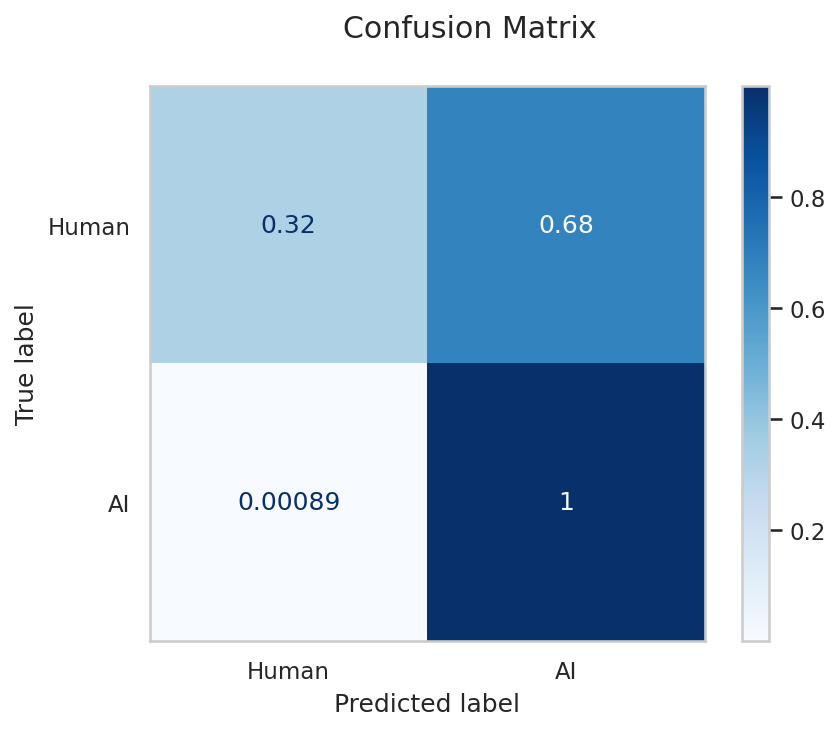
\includegraphics[width=\linewidth]{results/lora_raid_kaggle_4/confusion_matrix.png}
        \caption{OOD (Kaggle test set)}
    \end{subfigure}
    \caption{LoRA with $r{=}4$ evaluated in-domain and OOD.}
    \label{fig:best_model}
\end{figure}

% --- Hypothesis evaluation (6 pts) ---
\subsection{Hypothesis Evaluation}

\paragraph{H1: Confirmed (marginally).}
Full fine tuned RoBERTa has 99.95\% accuracy   compared to 99.74\% for TF-IDF+SVM and 95.64\% for GLTR+SVM. While the hypothesis is confirmed, it is so by a 0.21 margin. This reflects how easy the Kaggle dataset is for models to memorize.

\paragraph{H2: Confirmed}
RoBERTa fully fine tuned on RAID beats out kaggle-trained RoBERTa in OOD accuracy by achieving 50.22\% (macro-F1 0.45) compared to 42.79\% (macro-F1 0.37) which is a 7.4\% improvement hence confirming that training diversity aids OOD performance. As a side note, GLTR trained on Kaggle had an even better OOD performance (56\%)

\paragraph{H3: Confirmed}
LoRA-8 matches full fine tuned RoBERTa within 1 point in-domain on RAID wita macro f! of 0.92 compared to 0.93. LoRA-4 outperforms every tested model on OOD evaluations and beats full finetuning by 13 macro-F1 points (0.58 compared to 0.45). This confirms that LoRA with low rank acts as an effective regularizer. The concave shape observed in Figure \ref{fig:rank_sweep} confirms that there is a sweet spot below which the model underfits and above which OOD transfer collapses despite high in-domain performance. 

\section{Conclusion}

\subsection{Discussion and Limitations}
Our main finding is that great in-domain accuracy is a poor marker for real world performance when it comes to transformer based detectors. This is evident by how all methods tested achieve near perfect accuracy in-domain on Kaggle yet fail when evaluated OOD. This failure was consistent across all model despite major architectural differences, with TF-IDF, GLTR, and RoBERTa all demonstrating the same collapse by defaulting to generating false positives adn driving human recall to zero in OOD evaluations. This indicated that the problem was in the training data. We proved that what really promises OOD improvements in transformer based detectors is training set diversity (H2) and parameter-efficient adaptation (H3). Employing a diverse training set alone by switching from Kaggle to RAID improved OOD macro-F1 from 0.37 to 0.45 for full fine tuned RoBERTa. LoRA ($r{=}4,\alpha=8$) trained on RAID achieves the highest OOD macro-F1 of 0.58 while effectively training just 0.12\% of the parameter compared to full fine tuning of RoBERTa yet outperforms it by 13 points. This reinforces that PEFT acts as a regularizer and prevents memorization of source specific artifacts. The concave relationship between number of parameters and OOD performance further supports that if we reduce parameters too much, the model underfits while too many trainable parameters cause overfitting behavior.

However, our project has several limitations. We evaluate on only two datasets so generalization to other domains such as scientific writing or journalism is not guaranteed. We also only trained each model for only 4 epochs and did not conduct hyperparameter tuning of any kinds besides LoRA rank sweeps which themselves were limited to only 3 different ranks. Furthermore, we only tested one architecture with LoRA (RoBERTa) and what we observed might not transfer to other more sophisticated architectures. Finally, the biggest weakness of our study is that we do not test our approach on adversarial attacks such as paraphrasing or style transfer which is actually a very realistic threat model for detectors that are deployed.
\subsection{Future Work}
Several concrete directions for future investigation arise from our results. First, and most important of which is domain adversarial training which could in theory encourage the encoder to learn patterns that are embedded in both AI and human written text, potentially improving OOD transfer beyond what PEFT could achieve. Second, an approach to training which mixes different datasets or augmenting the training data may be able to rain the model to tackle domain shift further reducing transfer gap. Third, expanding the rank sweep to additional values could also lead to fruitful observations. Also, testing other architectures such as DeBERTa or Longformer would confirm whether the concave relation between parameters and OOD accuracy generalizes. Moreover, testing against adversarial attacks such as paraphrasing and
style transfer is a critical next step. Finally, a thorough study of ensembles and different loss objectives such as intrinsic dimensionality scoring, which has been shown by \cite{tulchinskii2023intrinsic} to seperate human from AI text without supervised training, could boost our supervised approach even further
\newpage
\begin{thebibliography}{10}

\bibitem[Devlin et~al.(2019)]{devlin2019bert}
Jacob Devlin, Ming-Wei Chang, Kenton Lee, and Kristina Toutanova.
\newblock {BERT}: Pre-training of deep bidirectional transformers for language understanding.
\newblock In \emph{Proceedings of NAACL-HLT}, 2019.

\bibitem[Dugan et~al.(2024)]{dugan2024raid}
Liam Dugan et~al.
\newblock {RAID}: A shared benchmark for robust {AI} detection.
\newblock Hugging Face dataset, 2024.

\bibitem[Gehrmann et~al.(2019)]{gehrmann2019gltr}
Sebastian Gehrmann, Hendrik Strobelt, and Alexander~M. Rush.
\newblock {GLTR}: Statistical detection and visualization of generated text.
\newblock In \emph{Proceedings of ACL: System Demonstrations}, pp.\ 111--116, 2019.

\bibitem[Guo et~al.(2023)]{guo2023close}
Bin Guo et~al.
\newblock How close is {ChatGPT} to human experts?
\newblock \emph{arXiv:2301.07597}, 2023.

\bibitem[Hu et~al.(2022)]{hu2022lora}
Edward~J. Hu et~al.
\newblock {LoRA}: Low-rank adaptation of large language models.
\newblock In \emph{ICLR}, 2022.

\bibitem[Liu et~al.(2019)]{liu2019roberta}
Yinhan Liu et~al.
\newblock {RoBERTa}: A robustly optimized {BERT} pretraining approach.
\newblock \emph{arXiv:1907.11692}, 2019.

\bibitem[Mitchell et~al.(2023)]{mitchell2023detectgpt}
Eric Mitchell et~al.
\newblock {DetectGPT}: Zero-shot machine-generated text detection using probability curvature.
\newblock \emph{arXiv:2301.11305}, 2023.

\bibitem[Thite(2026)]{thite2026kaggle}
Sunil Thite.
\newblock {LLM} -- Detect {AI} Generated Text Dataset.
\newblock Kaggle, 2026.

\bibitem[Uchendu et~al.(2021)]{uchendu2021turingbench}
Adaku Uchendu et~al.
\newblock {TURINGBENCH}: A benchmark environment for {T}uring test.
\newblock In \emph{Findings of EMNLP}, pp.\ 2001--2016, 2021.

\bibitem[Tulchinskii et~al.(2023)]{tulchinskii2023intrinsic}
Eduard Tulchinskii, Kristian Kuznetsov, Laida Kushnareva, Daniil Cherniavskii,
Serguei Barannikov, Irina Piontkovskaya, Sergey Nikolenko, and Evgeny Burnaev.
\newblock Intrinsic dimension estimation for robust detection of {AI}-generated texts.
\newblock In \emph{Advances in Neural Information Processing Systems (NeurIPS)}, 2023.

\end{thebibliography}

% ===========================================================================
% TEAM CONTRIBUTIONS  (4 pts — not in page limit)
% ===========================================================================
\newpage
\section*{Team Contributions}

\begin{table}[h]
\centering
\begin{tabular}{@{}lp{10cm}@{}}
\toprule
Member & Contributions \\
\midrule
Joseph Souaiby & Data preprocessing and splitting pipeline, GLTR baseline implementation, RoBERTa full fine-tuning on Kaggle and OOD evaluation on RAID, introduction, related work, hypothesis evaluation, discussion and limitations, and future work sections, proofreading. \\
\midrule
Huzaifah Wasim & Data preprocessing and splitting pipeline, TF-IDF baseline implementation, RAID RoBERTa and LoRA fine-tuning, problem formulation, method/approach, data, experiments and results sections, project coordination. \\
\bottomrule
\end{tabular}
\end{table}

\end{document}